\mode<all>
% Incluyo los paquetes necesarios.
% para no tener problemas con acentos etc.
\usepackage[utf8]{inputenc}
% en español
\usepackage[spanish]{babel}
%matemática
\usepackage{amsmath}
% este no se si hace falta pero por las dudas
\usepackage{graphicx}
% para incluir peliculas
\usepackage{multimedia}
% para usar segunda pantalla
\usepackage{pgfpages}
\usepackage{pgf}
% para hacer dibujitos
\usepackage{tikz}
\usetikzlibrary[automata,calc,arrows,decorations.pathmorphing,backgrounds,shapes,
patterns,positioning,fit,petri,overlay-beamer-styles]
\tikzstyle{every picture}+=[remember picture]
%recuadros sencillos
%\usepackage{tcolorbox}
% enumeradores intercambiables
\usepackage{enumerate}
% para subtitulos en figuras
\usepackage{subcaption}
%listings for code input
\usepackage{listings}
%verbatim input from file!
\usepackage{verbatim}
\usepackage{fancyvrb}
% para modificar los encabezados y pies de página.
%\usepackage{fancyhdr}
%\pagestyle{fancy}
\usepackage{standalone}

\definecolor{codegreen}{rgb}{0,0.6,0}
\definecolor{codegray}{rgb}{0.5,0.5,0.5}
\definecolor{codepurple}{rgb}{0.58,0,0.82}
%\definecolor{backcolour}{rgb}{0.95,0.95,0.0.1}

\lstset{
    basicstyle=\fontsize{8}{10}\selectfont\ttfamily, 
    backgroundcolor=\color{Beige},   
    frame=lines,
    commentstyle=\color{codegreen},
    keywordstyle=\color{magenta},
    numberstyle=\tiny\color{codegray},
    stringstyle=\color{codepurple},
    breakatwhitespace=false,         
    breaklines=true,                 
    captionpos=b,                    
    keepspaces=true,                 
    numbers=left,                    
    numbersep=5pt,                  
    showspaces=false,                
    showstringspaces=false,
    showtabs=false,                  
    tabsize=4
}



%\mode<presentation>{
% para ver las notas con la presentacion.  
%\setbeameroption{hide notes}
%para dejar las notas en la segunda patnalla
%}

% incluyo los beamercolors
%%%%%%%%%% BEAMERCOLORS
% el recuadro para el titulo
\setbeamercolor{title}{fg=white,bg=Purple}
% el recuadro para el subtitulo
\setbeamercolor{subtitle}{fg=white,bg=DarkOliveGreen}
% los títulos de las secciones tienen su colorinche:
\setbeamercolor{sectionbox}{fg=white,bg=Purple}
% cada diapositiva tendrá su color de título.
\setbeamercolor{frametitle}{fg=white,bg=ForestGreen}
% el título de las secciones tienen también su color. 
\setbeamercolor{sectiontitle}{fg=white,bg=violet}

%%%% CUSTOM BEAMERCOLORS
% estos cuadros los defino para ubicar al lector en los temas que se tratan
% son los cuadritos que aparecen arriba del título. 
\setbeamercolor{structure0}{fg=white,bg=gray}
\setbeamercolor{structure1}{fg=black,bg=DarkGray}
\setbeamercolor{structure2}{fg=black,bg=lightgray}
% defino un cuadro para usar en alguna oportunidad, creo que para titulos. 
\setbeamercolor{whitebox}{fg=black,bg=white}
% un cuadro para resaltar
\setbeamercolor{highlight1}{fg=black,bg=Gold}

% beamer colors for headers and etc.
\setbeamercolor{header1}{fg=white,bg=Blue}
\setbeamercolor{header2}{fg=black,bg=Red}
\setbeamercolor{header3}{fg=black,bg=ForestGreen}

%code block
\setbeamercolor{codeblock}{fg=Blue, bg=Beige}
\setbeamerfont{codeblock}{family=\ttfamily,size=\scriptsize}


%incluyo el tema y modificaciones
%%% BEAMER THEME
% el tema 'boxes' es igual al default pero permite definir boxes de estructura 
% a mano. 
\mode<presentation>{
  \usetheme{boxes}
  % los boxes que identifican lo que se esta leyendo
    % box de la izquierda: la materia (subtitulo)
    \addheadbox{structure2}{\quad \tiny \insertshortsubtitle}
  %  box del medio en cabecera, el titulo de la clase
    \addheadbox{structure0}{\quad \tiny  \inserttitle \quad } 
  % box en a la derecha , eltítulo de la sección. 
    \addheadbox{structure1}{\quad \tiny \insertsection}
}
% tema interno y de colores para las diapositivas normales. 
\useinnertheme{rectangles}
\usecolortheme{dove}
% la fuente de las ecuaciones
\usefonttheme[onlymath]{serif}

% entorno codeblock para meter piezas de código.
% el color se definió en BEAMERCOLORS

\newenvironment{codeblock}
{
  \begin{beamercolorbox}{codeblock}
    \usebeamerfont{codeblock}
}
{
  \end{beamercolorbox}
}



% modifico los temas
  \titlegraphic{%
\includegraphics[width=0.25\textwidth]{./PREAMBLE/logo-isabt25.png}
                
\includegraphics[width=0.25\textwidth]{./PREAMBLE/logo-isabato.png}
  		\hfill
		
\includegraphics[width=0.25\textwidth]{./PREAMBLE/ISOLOGOCNEA.png}
		\hfill
  		
\includegraphics[width=0.25\textwidth]{./PREAMBLE/unsam-horizontal.png}}

\mode<presentation>{
\setbeamertemplate{title page}[center]
{
  %
\includegraphics[width=0.25\textwidth]{./PREAMBLE/ISOLOGOCNEA.png}
  \inserttitle
  \insertsubtitle
  \insertauthor
  \insertinstitute
%  \inserttitlegraphic
}
}


% defino el template para las dapositivas con los titulos de las secciones. 
%es una recetita que saqué de algun lado. 
\setbeamertemplate{section page}{
  \begin{beamercolorbox}[ht=5ex,dp=1ex,wd=\paperwidth,center]{sectionbox}
    \begin{centering}
     \usebeamerfont{section  title} \insertsection 
    \end{centering}
  \end{beamercolorbox}
}
\AtBeginSection[]{
  \begin{frame}[plain]
    \begin{center}
    \quad \inserttitle \quad  
    \end{center}
    \sectionpage
  \end{frame}
}

% remover los simbolos de navegacion
% porque sacan espacio 
\mode<presentation>{
\setbeamertemplate{navigation symbols}{}
\setbeamertemplate{footline}[page number]
% me gustan los titulos a la derecha
\setbeamertemplate{frametitle}[default][right]%{
}
\mode<handout>{
 \setbeamertemplate{headline}{}
 \setbeamertemplate{frametitle}{}
 \setbeamertemplate{background}{
   \tikz\node [rectangle,minimum width=0.995\paperwidth,
   minimum height=0.995\paperheight,draw,anchor=south west,
   line width=2pt]  {};
 }
 \setbeamertemplate{footline}{}
}
% aparentemente el siguiente beamertemplate
%se ejecuta en modo artículo. habría que ver
%la forma de sacale probecho. 
% notar que vale solo para las framesque se incluyen 
% directamente en el artículo y no vale para 
% \includeslide.
% \setbeamertemplate{frame begin}
% \setbeamertemplate{frame end}


% no se si es el mejor lugar para definirlo, 
% pero las \includeslides deben quedar fijas al
% tamaño de la página:

%\mode<article>{
%\renewcommand\includeslide[1]{
%  \includeslide[width=\textwidth]{#1}
%}
%}

% defino el template para la diapositiva del título

%%%%%%%%%%%%%%%%%%%%%%%%%%%%%%%%
% Defino la Clase
%%%%%%%%%%%%%%%%%%%%%%%%%%%%%%%%
\subtitle[Modelización 2020]{ Modelización de Propiedades y Procesos 2021 }
\author{Ruben Weht\inst{1,2} \and Mariano Forti\inst{1,3} }
\institute{
%  \inst{1}Instituto de Tecnología Prof. Jorge Sabato
%  \and
  \inst{1}Fisica del Sólido, Edificio TANDAR, \url{weht@cnea.gov.ar},
  interno 7104
  \and
  \inst{2}División Aleaciones Especiales, Edificio 47 (microscopía),
  \url{mforti@cnea.gov.ar}, interno 7832
}

\mode<presentation>{\date{}}

\mode<article>{
  \date{
    \small
%  \textsuperscript{1} Instituto de Tecnología Prof. Jorge Sabato\\
  \textsuperscript{1}Fisica del Sólido, Edificio TANDAR, \url{weht@cnea.gov.ar},
  interno 7104 \\
  \textsuperscript{2}División Aleaciones Especiales, Edificio 47 (microscopía),
  \url{mforti@cnea.gov.ar}, interno 7832
}

%defino los encabezados y pies de págna para
% dodo el documento en función de la materia y la
% clase.
%\fancyhead[L]{\tiny Modelización de Materiales 2019}
%\fancyhead[R]{\tiny \leftmark}
}

\title{
  \mode<article>{

\includegraphics[height=1cm]{./PREAMBLE/logo-isabt25.png}
\hfill

\includegraphics[height=1cm]{./PREAMBLE/ISOLOGOCNEA.png}
\hfill
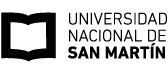
\includegraphics[height=1cm]{./PREAMBLE/logo-unsam.png}
\\}  Método de las Difrerencias Finitas }
\subject{Repaso de Diferencias Finitas, Ayudas para el ejercicio 1 de la guía}
\keywords{Modelizacion 2020, Diferencias Finitas  }
% Inicia el documento.
\begin{document}

% Título de la clase. 
\mode<presentation>{
\begin{frame}[plain]
\titlepage
\end{frame}
}

\mode<article>{
\maketitle
}
\mode<all>

\section{Problema de la chapa}
\mode<article>

Vamos a encarar el problema presentado en la Figura \ref{FiuguraPresentacionProblema}. 
se tiene una chapa dispuesta bajo condiciones de contorno tales que sus lados se 
encuentran a temperaturas fijas  $T_A$, $T_B$, $T_C$, $T_D$.

Queremos obtener la distribución de temperatura dentro 
del recinto de la chapa, en condiciones estacionarias, 
es decir, cuando las temperaturas de no varían en ningún 
punto del recinto. Por lo tanto, podemos elegir el 
modelo físico a resolver. La ecuación diferencial 
que rige el problema es la ecuación de Poison, que es 
la ecuación de transferencia térmica homogénea. 

  \begin{equation}
    \frac{\partial ^2 T_{(x,y)}}{\partial x ^2}
    +
    \frac{\partial ^2 T_{(x,y)} }{\partial y ^2}
    =0
    \label{EqEcuacionPoisson}
  \end{equation}

Debido a que los contornos del recinto donde debemos
resolver la ecuación \ref{EqEcuacionPoisson} son los adecuados,
elegimos utilizar el método de \textbf{Diferencias Finitas}. 


\begin{figure}
  \includeslide[width=\textwidth]{FrameProblema}
  \caption{Presentación del Problema. Chapa bidimensional 
  de conductividad térmica finita, cuyos bordes se encuentran 
  a temperaturas constantes finitas $T_A$, $T_B$, $T_C$, $T_D$}
  \label{FiuguraPresentacionProblema}.
\end{figure}

\mode<all>

\mode*

\begin{frame}<presentation:1|article:0>[label=FrameProblema]
  \frametitle<1>{Presentación del Problema}
  \frametitle<2>{Bordes a temperatura Fija}
%  \begin{tikzpicture}[overlay]
%    \draw [draw,thick,pattern=north east lines] (4.9,-3.1) rectangle (9.1,1.1);
%    \draw [draw,line width=2pt,anchor=base,fill=white] (5,-3) rectangle (9,1);
%    \draw [<->, >=latex, line width = 2pt ]
%    (2,-1) node [anchor=south] { $y_j$ }  -- (2,-3) -- (4,-3) node [anchor=south] {$x_i$};
%  \end{tikzpicture}
  \tikz[overlay] \node at (6,-1) {
    \includegraphics[width=9 cm]{./01-Problema/Figura01-01-Chapa.pdf}
  };

%  \begin{equation}
$$  \frac{\partial ^2 T_{(x,y)}}{\partial x ^2}
    +
    \frac{\partial ^2 T_{(x,y)} }{\partial y ^2}
    =0 $$
%  \end{equation}

\end{frame}

\mode<all>

\subsection{Discretización del Problema}
\mode<article>

El primer paso en este sentido consiste en discretizar 
el dominio de la chapa en un conjunto de puntos regularmente 
distribuídos. Al tratarse de un recinto cuadrado, este paso es trivial.

Para formar la grilla dividimos los lados sobre 
los ejes $x$ e $y$ del cuadrado en $N_x-1$ y $N_y-1$
segmentos iguales, determinando $N_x$ y $N_y$ puntos
equidistantes sobre cada uno. De las intersecciones
de las líneas paralelas a los lados que se 
extienden de los puntos formados se genera la grilla 
a usar, como se muestra en la Figura \ref{FiguraDiscretizacion}.
Puede verse inmediatamente que la cantidad de nodos
total de la grila es $N_x N_y$

\begin{figure}
  \includeslide[width=\textwidth]{FrameDiscretizacion}
  \caption{Grilla de discretización del dominio de la chapa\label{FiguraDiscretizacion}}
\end{figure}

%Supongamos por un instante que conocemos la distribución
%de temperaturas en la chapa.
Para poder asignar una temperatura a cada nodo de la grilla, 
debemos tomar una convención para numerarlos. La primera
intuición tiene que ver con una numeración de índices según 
las dos direcciones cartesianas $x$ e $y$. Necesitamos 
entonces dos índices $i$ y $j$, de manera que las 
temperaturas $T(x_i,y_j)$ para los nodos de la grilla
pueden representarse en forma matricial $T_{i,j}$.

Sin embargo, por razones que pronto quedarán claras, es 
conveniente tomar una numeración de un único índice $k$
para cada nodo.  
Con alguna arbitrariedad, puede tomarse una numeración
correlativa asignando $k=1$ al nodo del 
el vértice inferior izquierdo, hacia la 
derecha. En cada ``fin de línea'' se toma el índice 
siguiente para el primer nodo de la línea superior. 
Con esta convención, puede verse que los vértices 
de la chapa quedan identificados en función de las dimensiones
de la grilla elegida

\begin{equation}
  \begin{split}
    \text{Vertice inferior izquierdo:   } & k=1\\
    \text{Vertice inferior derecho:     } & k=N_x \\
    \text{Vertice superior izquierdo:   } & k=N_xN_y-N_x+1\\
    \text{Vertice superior derecho:     } & k=N_xN_y
  \end{split}
  \label{EqEcuacionesNumeracionVerticies}
\end{equation}

Ahora, las temperaturas de la barra 
pueden representarse en un \textbf{vector} 

\begin{equation} \label{EqEcuacionVectorT}
  \vec{T} = 
  \begin{pmatrix}
    T_1 \\ T_2 \\ \vdots \\ T_{Nx Ny}
  \end{pmatrix}
\end{equation}

Es conveniente encontrar una relación entre los sistemas
de índices. como $1 \leq i \leq N_x $ ; $1 \leq j \leq  N_y$, puede verse
fácilmente que dicha relación es

\begin{equation}\label{EqEcuacionRelacionIndices}
  \begin{aligned}
  k &= i + (j-1)N_x \\
  j &= floor \bigg( \frac{k-1}{N_x} +1  \bigg)\\
  i &= k - (j-1)N_x
  \end{aligned}
\end{equation}
donde la función $floor$ indica que debe tomarse la parte
entera inferior de su argumento. Por otro lado, las relaciones
de la ecuación \ref{EqEcuacionRelacionIndices} permite
relacionar ambas convenciones de índices en forma biyectiva, 
de manera que podamos relacionarlo
con la numeración de dos índices $i,j$ en forma unívoca.


Según el método de las diferencias fnitas, debemos
usar las versiones \emph{discretas} de las derivadas
segundas en la ecuación \ref{EqEcuacionPoisson}. 
Puede consultar la teórica para rescatar estas 
definiciones, pero aquí razonaremos en base a las
mismas, que las derivadas segundas pueden calcularse
a partir de las derivadas primeras. 

Para empezar por el problema más sencillo, busquemos la
segunda derivada parcial respecto de x como un cociente 
incremental de las derivadas primeras. 
Dado un nodo de 
numeración $k$ \emph{que no se encuentre en ningún borde
de la chapa}, notemos según nuestra convención el punto
siguiente hacia las $ x $ positivas es el número $k+1$, mientras
que el nodo hacia las $ x $ negativas es el $k-1$. Podemos
definir entonces las derivadas primera y segunda en el
nodo $k$-ésimo como 

\begin{equation}\label{EqEcuacionDerivadaX}
    \begin{aligned}
    \frac{\partial T}{\partial x} \Bigr\rvert _k &=
			   \frac{T_{k}-T_{k-1}}{\Delta x} &= dT_k  \\
    \frac{\partial^2 T}{\partial x^2} \Bigr\rvert _k &=
    \frac{dT_{k+1}- dT_k}{\Delta x}                  &= 
			   \frac{1}{\Delta x} \big(
			   \frac{T_{k+1}-T_k}{\Delta x}
			   -
			   \frac{T_{k}-T_{k-1} }{\Delta x}
			   \big)\\
    \Rightarrow  &= 
    \frac{T_{k+1} - 2T_k +T_{k-1} }{\Delta x ^2}
  \end{aligned}
\end{equation}

%  \label{EqDerivadaDiscretaX}
%\end{multline}

Para poder calcular la derivada segunda en la otra dirección 
debemos notar que es necesario tomar cocientes incrementales
de la temperatura hacia arriba y hacia abajo. Debe notar que 
para un nodo de índice $k$, el nodo de \emph{arriva} tiene 
el orden $k+N_x$. Haga el ejercicio de obtener la derivada 
segunda respecto de y

\begin{equation}\label{EqEcuacionDerivadaY}
    \frac{\partial^2 T}{\partial y^2} \Bigr\rvert _k 
    =
    \frac{T_{k+N_x} - 2T_k +T_{k-N_y} }{\Delta y ^2}
\end{equation}



\mode*

\begin{frame}<presentation>[label=FrameDiscretizacion]
  \frametitle{Discretización del Problema}
  \begin{columns}
    \column{0.6\textwidth}
    \includegraphics[width=\textwidth]{./01-Problema/01-Figura-Grilla.pdf}
%    \documentclass{standalone}
\usepackage[dvipsnames,x11names,svgnames]{xcolor}
\usepackage{tikz}
\usepackage{amsmath}
\usetikzlibrary{patterns,positioning,arrows}

\begin{document}

\tikzset{font={\fontsize{6pt}{10}\selectfont}}
  \begin{tikzpicture}
    \draw [draw,line width=0.025cm] (-2,-2) grid (2,2);
    \foreach \x in {-2,-1,0,1,2}
	\foreach \y in {-2,-1,0,1,2}
	   {
	     \draw [fill=black](\x,\y) circle (0.05cm) node (\x\y) {};
	     }
    
    \node [draw=none, anchor=north east ] at ( -2,-2 ) {$k=1$};
    \node [draw=none, anchor=south] at ( -2,2 ) {$k=1+(Ny-1)N_x$};
    \node [draw=none, anchor=north west ] at ( 2,-2 ) {$k=N_x$};
    \node [draw=none, anchor=south west ] at ( 2,2 ) {$k=N_x N_y$};
    \node [draw=none, anchor=south west ] (k) at ( 0,0 ) {$k$};
    \draw [->,>=latex,PineGreen,line width=0.5pt] (k) to [bend left] (10) 
    node [above] {$+1$} ;
    \draw [->,>=latex,PineGreen,line width=0.5pt] (00) to [bend right] (-10) node [above] {$-1$} ;
    \draw [->,>=latex,BrickRed,line width=0.5pt] (00) to [bend left] (01) node [left] {$+N_x$} ;
    \draw [->,>=latex,BrickRed,line width=0.5pt] (00) to [bend right] (0-1) node [left] {$-N_x$} ;
    \draw [->,>=latex,BrickRed,dashed] (00) to [bend right=30] (10);
    \draw [->,>=latex,BrickRed,dashed] (10) to [bend right=30] (20);
    \draw [->,>=latex,BrickRed,dashed] (-21) to[bend right=30] (-11);
    \draw [->,>=latex,BrickRed,dashed] (-11) to[bend left=30] (01);

    %\node [draw=none, anchor=south west ] (kr) at ( 1,0 ) {$k+1$};
    %\node [draw=none, anchor=south east ] (kl) at ( -1,0 ) {$k+1$};
    
  \end{tikzpicture}

\end{document}

    \column{0.5\textwidth}
\centering
$\frac{T_{k+1} - 2T_k +T_{k-1} }
  {\Delta x ^2} +
 \frac{ T_{k+N_x} - 2T_k +T_{k-N_y} }{ \Delta y^2 } =0 $

    \vspace{1cm}
    $ \vec{T}= \begin{pmatrix}
    T_1 \\ T_2 \\ \vdots \\ T_{Nx Ny}
     \end{pmatrix}$ 

  \end{columns}
\end{frame}

\mode<all>

\section{Matricialización del Probema}
\mode<article>
Siguiendo el método de las diferencias Finitas, 
sólo resta reemplazar las ecuaciones \ref{EqEcuacionDerivadaX} 
y \ref{EqEcuacionDerivadaY} en la \ref{EqEcuacionPoisson}. Puede
verse fácilmente\footnote{hágalo, ¡atrévase!} que \emph{para el 
conjunto de nodos del interior de la chapa } se puede escribir
la ecuación

\begin{equation}\label{EqEcuacionDiferenciasFinitas}
  \begin{aligned}
    \frac{T_{k+1} - 2T_k +T_{k-1} }
    {\Delta x ^2}    
    +
    \frac{T_{k+N_x} - 2T_k +T_{k-N_y} }
    {\Delta y ^2}
    &= 0 \\
    \beta ^2 T_{k-N_x}+T_{k-1} 
    - 2\big(1+\beta^2\big) T_k
    +T_{k+1} + \beta^2 T_{k+N_x} &= 0
  \end{aligned}
\end{equation}

donde se ha definido 
\begin{equation}\label{EqEcuacionBeta}
  \beta = \frac{\Delta x}{\Delta y}
\end{equation}

La ecuación 
\ref{EqEcuacionDiferenciasFinitas}
es válida para todos los nodos de índice
$k$ tal que siguiendo la biyección de la
ecuación \ref{EqEcuacionRelacionIndices}
se tiene que $0<i<N_x$ y $0<j<N_y$, donde
el uso del menor estricto refleja que
los nodos no estan en los bordes. 
Para los
nodos de los bordes debemos tomar una 
consideración especial. 

Aún en este caso general, podemos ver 
lo siguiente. Cada nodo interno de la chapa
cumple la ecuación \ref{EqEcuacionDiferenciasFinitas}. Si las 
temperaturas de los nodos están dispuestas en
el vector $\vec{T}$ de la ecuación \ref{EqEcuacionVectorT}
la ecuación diferencial surge de multiplicar
un vector fila por el vector columna $\vec{T}$.
El conjunto de ecuaciones para todos los $k$
internos genera entonces un sistema lineal 
cuyos coeficientes están bien determinados 
en la ecuación \ref{EqEcuacionDiferenciasFinitas},
como se muestra en la Figura \ref{FiguraCoeficientesMatriz}.

\begin{figure}
  \includeslide[width=\textwidth]{FrameCoeficientesMatriz}
  \caption{Ilustración de la construcción de los coeficientes de matríz
  para la fila $k$-ésima de la matriz del sistema lineal, para algún
  $k$ correspondiente a un nodo del interior de la chapa.
  \label{FiguraCoeficientesMatriz}}

\end{figure}
\mode*

\begin{frame}<presentation>[label=FrameEciacionInterior]
  \frametitle{Matricialización de la Ecuación Diferencial}
 $$\beta ^2 T_{k-N_x}+T_{k-1}- 2\big(1+\beta^2\big) T_k +T_{k+1} + \beta^2 T_{k+N_x} = 0$$

  \begin{columns}
    \column{0.6\textwidth}
    \begin{tikzpicture}[scale=1.5]
      \draw [thick] (-2,-2) grid (2,2) ;
      \foreach \x in {-2,-1,0,1,2}
        \foreach \y in {-2,-1,0,1,2}
	{
	  \draw [fill=black] (\x,\y) circle (1pt);
	  };
      \draw [dashed,OliveGreen,line width=2pt] (-1.5,-1.5) rectangle (1.5,1.5);
    \end{tikzpicture}

    \column{0.4\textwidth}
    %\begin{equation}
      \resizebox{2cm}{!}{$\big[\mathbf{M}\big] $}
$  \begin{pmatrix}
    T_1 \\ T_2 \\ \vdots \\ T_{Nx Ny}
  \end{pmatrix} 
  =  \vec{b} $
% \end{equation}
  \end{columns}

\end{frame}

\begin{frame}<presentation>[label=FrameCoeficientesMatriz]
  \frametitle{Coeficientes de Matriz}
  \centering
%  \framesubtitle{Para los nodos internos}
  \tikz [baseline] \node  (ecuacion) at (0,0)  {
    $\beta ^2 T_{k-N_x}+T_{k-1}- 
    2\big(1+\beta^2\big) T_k +T_{k+1} + \beta^2 T_{k+N_x} = 0$
  };

  \vspace{0.5cm}

\flushleft
  Fila $k$-esima: 

\centering

  \vspace{0.5cm}

  $M [k,:] = \Big[ \dotsi $ 
  \tikz[baseline] \node [anchor=base] (-b2) at (0,0) {$\beta^2$} ;
  $ \dotsi $
  \tikz[baseline] \node [anchor=base] (k-1) at (0,0) {$1$};
  $ \dotsi  $
  \tikz[baseline] \node [anchor=base] (diag) at (0,0) {$-2\big(1+\beta^2\big)$};
  $ \dotsi $
  \tikz[baseline] \node [anchor=base] (k+1) at (0,0) {$1$};
  $\dotsi $  
  \tikz[baseline] \node [anchor=base] (b2) at (0,0) {$ \beta^2$} ;
  $ \dotsi \Big]$
  \tikz[overlay,->] \draw [blue] (-b2.south west) -- ($(-b2)-(2,2)$)  node[text=black,anchor=north] {$k-N_x$};
  \tikz[overlay,->] \draw [blue] (k-1.south)      -- ($(k-1)-(1,2)$)  node[text=black,anchor=north] {$k-1$};
  \tikz[overlay,->] \draw [blue] (diag.south)     -- ($(diag)-(0,2)$) node[text=black,anchor=north] {$k$};
  \tikz[overlay,->] \draw [blue] (k+1.south)      -- ($(k+1)-(-1,2)$) node[text=black,anchor=north] {$k+1$};
  \tikz[overlay,->] \draw [blue] (b2.south)       -- ($(b2)-(-2,2)$)  node[text=black,anchor=north] {$k+N_x$};

  \vspace{3cm}

  \hfill  \tikz[baseline]  \node (b0) at (-0.5,0) {$b_k  = 0$}; 
  \hspace{1cm} \tikz[baseline,fill=none]  \node (help) at (0,0) {};
  \tikz[overlay] \draw [->,>=latex,blue] (ecuacion.east) -| (help.west) -- (b0.east);
 
\end{frame}

\mode<all>

\section{Condiciones de Contorno}
\subsection{ Borde a Temperatura Fija }
\mode<article>

Para describir el problema en forma completa, las 
condiciones de contorno deben ser dadas. Comencemos
por el caso más sencillo en el que se conoce el 
valor de la función incógnita en el borde del
recinto de integración, tal como se mostró en
la figura \ref{FiuguraPresentacionProblema}.

Para poder expresar estas condiciones de contorno
en nuestro modelo computacional, debemos pensar 
primero en la numeración que recibirán los nodos
de cada borde. podemos entonces tomar los
vectores de índices que los describen. Retomando
la numeración descrita en la Figura \ref{FiguraDiscretizacion}, 
podemos escribir los siguientes vectores

\begin{equation}\label{EqNumeracionBordes}
  \begin{split}
  k_A &= \Big[1,1+Nx, \dotsi ,1+(N_y -1)N_x\Big]\\
  k_B &= \Big[Nx, 2N_x,  \dotsi , N_yN_x\Big]\\
  k_C &= \Big[1,2,\dotsi,N_x]\\
  k_D &= \Big[1+(N_y-1)N_x,2+(N_y-1)N_x,\dotsi, N_x N_y]
  \end{split}
\end{equation}

Para cualquiera de los nodos cuyo índice $k$ puede
encontrarse en alguno de los vectores de la ecuación
\ref{EqNumeracionBordes}, se tiene que la ecuación 
que \emph{deben cumplir} es

\begin{equation}\label{EqEcuacionesTFija}
  T_{k \in k_A} = T_A ;  T_{k \in k_B} = T_B ; T_{k \in k_C} = T_C ; T_{k \in k_D} = T_D
\end{equation}

Estas últimas condiciones son triviales de conseguir si 
se cambian los coeficientes de las filas de la matríz
correspondientes y el vector $\vec{b}$ como se 
muestra en la Figura \label{FiguraContornoTFija}. Se
muestra que como la ecuación se ha cambiado por 
la \ref{EqEcuacionesTFija}, solo el coeficiente 
de la diagonal es distinto de cero. El resto
de los coeficientes en las columnas no diagonales
es nulo ya que a la derecha del igual los nodos
con $ k' \neq k $ aparecen solo en forma implícita 
multiplicados por cero. 

\begin{figure}
  \includeslide[width=\textwidth]{FrameContornoTFija} 
  \caption{Coeficientes de matriz para los nodos
  en cualquiera de los bordes del recinto del problema.
  \label{FiguraContornoTFija}}
\end{figure}


\mode*

\againframe<2>{FrameProblema}

\begin{frame}<presentation>[label=FrameContornoTFija]
  \frametitle{Borde a temperatura fija}

  \begin{columns}
    \column{0.5\textwidth}
    \begin{tikzpicture}
      \draw [line width=1pt] (-2,-2) grid (2,2);
      \foreach \x in {-2,-1,0,1,2}
            \foreach \y in {-2,-1,0,1,2}
	    {
	      \draw [fill=black] (\x,\y) circle (2pt);
	      };
       	
       \foreach \y in {-2,-1,0,1}
       {
	 \draw [BrickRed,->,>=latex,line width=1pt] 
	 (-2,\y) .. controls (-2.5,\y+0.5) ..  (-2,\y+1);
	 };

	 \draw [OliveGreen,dashed,line width=2pt] (-2.5,-2.5) rectangle (-1.5,2.5);
    \end{tikzpicture}
    
    \column{0.5\textwidth}

    \tikz[baseline]\node (cc) at (0,0) {$T_{k_A}=T_A$}; \hfill

    
     \mode<handout>{$k_A = \big[ 1:Nx:1+(N_y-1)N_x\big]$} \mode<beamer>{$k_A = ?$ Algun Rango ...}

    \vspace{0.5cm}

    $M_{k_A} ^{fija} = \Big[ \dotsi$ 
    \tikz[baseline] \node (diag) at (0,0) {$1$};
    $\dotsi \Big]$
    \tikz[overlay] \draw [blue, ->, >=latex ] (diag) -- ($(diag)-(0,1)$) 
    node [anchor=north,text=black] { $k_A$};

    \vspace{2cm}

    \tikz[baseline] \node (bk) [text=black,anchor=east] {$b_k = T_A$};


    \tikz[overlay] \draw [blue,->,>=latex] (cc) -| ($(bk)+(5,0)$) -- (bk); %-- (bk);

  \end{columns}

\end{frame}

\mode<all>

\subsubsection{Vértices} 
\mode<article>

El caso de los vértices debe ser tratado en forma separada. 
esto se debe a que según la definición de los bordes en 
la ecuación \ref{EqNumeracionBordes}, los nodos en los 
vértices pueden pertenecer a dos bordes simultáneamente.
Por ejemplo el nodo $k=1$ pertenece a $k_A$ y a $K_C$. 

Pueden tomarse varias estrategias para atacar estos 
problemas. Podemos tomar preferencia por alguno de 
los bordes. Entonces la lógica que adoptaremos 
debe evaluar primero si los nodos están en los
bordes según la preferencia dada. 

Otra alternativa es que la lógica de la solución 
evalúe primero si el nodo está en algún borde, se 
le asigne alguna condición de contorno específica.
Una vez descartada la pertenencia a todos los vértices,
evaluar la pertecia a los bordes. 
En este úlimo caso es sencillo asignar por ejemplo
el promedio de las temperaturas de los bordes 
subyacentes al vértice, por ejemplo.

\mode*
\begin{frame}<presentation:0>[label=FrameEmpty1]
  \frametitle{}
\end{frame}
\mode<all>

\section{Lógica}
\mode<article>

Sabiendo los valores de los coeficientes de la matriz que 
representa a nuestra ecuación diferencial, podemos trazar la 
lógica de nuestro modelo computacional.

Cuando inicie el estudio del problema, no use tamaños de grillas 
grandes. Utilice la mínima grilla posible, por ejemplo
$N_x = N_y = 3$ para poder interpretar los resultados 
en forma legible. 

\mode*

\begin{frame}<presentation>[label=FrameLogicaEnumerate]
  \frametitle{Lógica del programa}
  
\begin{enumerate}
    \item<+-> Recorrer todos los valores posibles para el índice k, es decir los nodos
    \item<+-> decidir si el nodo está en un borde o en el interior de la chapa
    \item<+-> llenar la fila correspondiente de la matriz y al vector $\vec{b}$
      en consecuencia.
    \item<+-> resolver el sistema lineal
    \item<+-> Graficar !
\end{enumerate}

\end{frame}

\begin{frame}<presentation>[label=FrameLogica]
  \frametitle{Lógica del modelo}
  \begin{tikzpicture}[every node/.style={
      rectangle, minimum size=1cm, draw, thick,
      align=center, font=\ttfamily
    },
    every path/.style={ >=latex },
    node distance=1.5cm and 1.5cm]

    % column 1
    \node (start) {Leer Condiciones\\de Contorno };
    \node[below of=start] (fork) {$1\leq k \leq N_x N_y $};
    \node [below of=fork] (vertex) {$k \in k_A,k_B, k_C,k_D$ ?};

    %column 2
    \node [right=of start] (matrix) {Armar la\\matriz};
    \node [below of=matrix] (sizes) {$N_x , N_y$};
    \node [below of=sizes](matcc) {
      \scalebox{0.5}{$ M[ k, :] = [\dotsi , 0,  1,0,\dotsi] $ } };
    \node [below of=matcc] (eqint) { \scalebox{0.5}{
      $M[k,[k-N_x,k-1,k,k+1,k+N_x]]=[ \beta ^2 , 1 , 2\big(1+\beta^2\big),  1 \beta^2]$
    }
    };

    % column 3
    \node [right=of matrix] (solve) {resolver el\\sistema};

    %column 4
    \node [right=of solve] (graph) {graficar};

    %row 1
    \draw [->] (start) -- (matrix);
    \draw [->] (matrix) -- (solve);
    \draw [->] (solve) -- (graph);
    \draw[->] (vertex) -- (matcc) node [midway,above,draw=none] {Si};
    \draw[->] (vertex.south) |- (eqint.west) node [midway,left,draw=none] {No};
    
  \end{tikzpicture}
\end{frame}

\mode<all>

\section{Resultados con temperaturas Fijas}
\mode<article>
Una vez se haya armado la matriz, debe resolver el sistema lineal
\begin{equation}\label{EqEcuacionSistemaLineal}
  \mathbf{A} \vec{T} = \vec{b}
\end{equation}

Utilice las subrutinas especializadas del lenguaje que haya elegido 
para implementar el método. En la figura \ref{FiguraCodeblockSolve}
se muestran las órdenes en \texttt{Matlab} y en \texttt{python}. 
Por el otro lado, en la Figura \label{FiguraResultadoTfija} se 
muestra las curvas de nivel obtenidas imponiendo temperaturas
arbitrarias en los bordes. Al mismo tiempo se muestran los ajustes
lineales de los tiempos de ejecución de las subrutinas de 
resolución del sistema lineal. 

Se usaron programas redactados en \texttt{python} y \texttt{FORTRAN}
como ejemplo de los dos tipos de lenguajes compilables y no compilables.
Por un lado, lo tiempos en \texttt{FORTRAN} son menores que en
\texttt{python}. Por otro lado, los tiempos medidos para la 
ejecución de la solución del sistema en \texttt{python} 
ajustan mal al modelo lineal, lo que se evidencia en el
mayor error en los parámetros de ajuste. Esto se debe a que
el programa \texttt{FORTRAN} se ha compilado para que la ejecución 
se implemente en un ejecutable binario que interactúa con 
la CPU `con menos intermediarios`, por decirlo de alguna 
manera. Por otro lado, el intérprete \texttt{python} 
debe pasar el programa a lenguaje de máquina en tiempo
de ejecución, lo que evidentemente insume un 
tiempo considerable.

\begin{figure}
  \includeslide[width=\textwidth]{FrameCodeblockSolve}
  \caption{Órdenes \texttt{Matlab} y \texttt{python} para 
  resolver sistemas lineales\label{FiguraCodeblockSolve} }
\end{figure}

\begin{figure}
  \includeslide[width=\textwidth]{FrameResultadoTfija}
  \caption{Resultado en el caso de bordes a temperatura fija
  \label{FiguraResultadoTfija}}
\end{figure}
%
\mode*
\begin{frame}<presentation>[label=FrameCodeblockSolve]
  \frametitle{Códigos de solución}
  
  \begin{columns}[T]
    \column{0.4\textwidth}
Resolver: \hfill    \texttt{Matlab}
    \column{0.6\textwidth}
  \begin{codeblock}
    \verbatiminput{./codexamples/solve.m}
  \end{codeblock}
  \end{columns}

  \begin{columns}[T]
    \column{0.4\textwidth}
\hfill    \texttt{ python }
    \column{0.6\textwidth}
    \begin{codeblock}
      \verbatiminput{./codexamples/solve.py}
    \end{codeblock}
  \end{columns}

  \begin{columns}[T]
    \column{0.4\textwidth}
  Graficar: \hfill \texttt{Matlab}
    \column{0.6\textwidth}
    \begin{codeblock}
      \verbatiminput{./codexamples/contourf.m}
    \end{codeblock}
  \end{columns}

  \begin{columns}[T]
    \column{0.4\textwidth}
    \hfill \texttt{python}
    \column{0.6\textwidth}
    \begin{codeblock}
      \verbatiminput{./codexamples/contourf.py}
    \end{codeblock}
  \end{columns}


\end{frame}
%
%
\begin{frame}<presentation>[label=FrameResultadoTfija]
  \frametitle{Resultado primero}
  \centering
    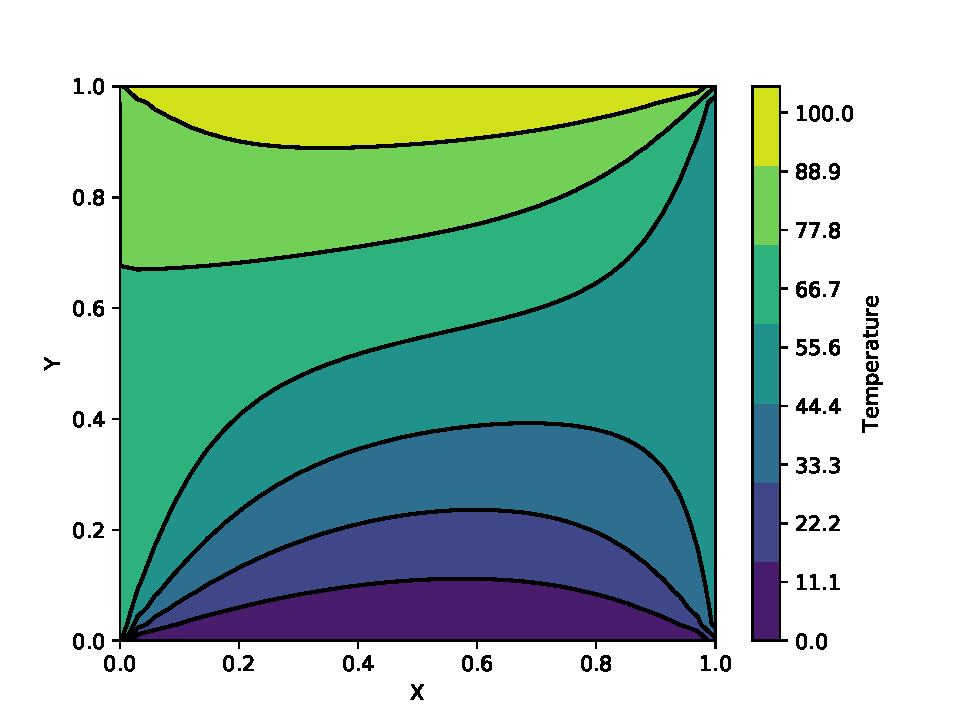
\includegraphics[width=0.4\textwidth,bb=0cm 0cm 14.5cm 12cm,clip,page=1]
    {./DATA/Temperaturas-Flujos-1.pdf}
    \hspace{1cm}
    \includegraphics[width=0.5\textwidth]{./DATA/tiempos.pdf}

\end{frame}
\mode<all>

\section{Cálculo de Flujos}
\mode<article>

Una vez obtenida la distribución de temperaturas,
podemos medir, por ejemplo, los flujos de calor 
que de ella se derivan.  Como sabemos, los flujos de
calor son proporcionales a la derivada primera de 
la temperatura. En los nodos interiores, es posible
aproximar esta derivada por un cociente incremental
centrado como se esquematiza en la figura \ref{FiguraFlujosCalorAdentro}.
 Sin embargo, en los bordes es necesario tomar
 algunos cuidados. Por ejemplo, es posible optar
 por tomar cocientes incrementales hacia la derecha
 para los nodos en el bordeizquierdo, etc. 

Pueden utilizarse varios métodos para visualizar 
los campos vectoriales como el flujo, pero en 
general es necesario ejecutar una instrucción 
cuyos argumentos serán las posiciones a las que
corresponden cada vector, y las componentes 
$x$ e $y$ para cada punto del recinto calculado.
El resultado se muestra en la Figura \ref{FiguraResultadosFlujos}

\begin{figure}
  \includeslide[width=\textwidth]{FrameFlujosCalorAdentro}
  \caption{Derivadas Primeras para los nodos interiores 
  y del borde. \label{FiguraFlujosCalorAdentro}}
\end{figure}

\begin{figure}
  \includeslide[width=\textwidth]{FrameResultadosFlujos}
  \caption{Resultado final incluyendo el flujo de calor para 
  las condiciones de borde de temperatura \label{FiguraResultadosFlujos}
  }
\end{figure}

\mode*
\begin{frame}<presentation>[label=FrameFlujosCalorAdentro]
  \frametitle{Cálculo de los Flujos de Calor}
    \tikzset{dT/.style={->,>=latex,line width=2pt}}
    \tikzset{dy/.style={alt=<beamer>{draw=Blue},alt=<handout>{draw=DarkRed}}}
    \tikzset{dx/.style={draw=Blue}}
  \begin{columns}
    \column{0.7\textwidth}
    \centering
    \begin{tikzpicture}
    \draw [line width=1pt] (-2,-2) grid (2,2);
    \foreach \x in {-2,...,2}
    	\foreach \y in {-2,...,2}
	{
	  \draw [fill=black] (\x,\y) circle (2pt);
	  }
      \draw [draw=none,fill=black,minimum height=1pt] (0,0) circle (2pt); 
      \draw [ dashed, draw=DarkGreen, line width=2pt ] (-1.5,-1.5) rectangle (1.5,1.5);
      \draw<2> [dT, draw=Blue ] (-1,0) -- (1,0) ;
      \draw<3> [dT,dy] (0,-1) -- (0,1) ;
      \node [draw=none,fill=black, circle,minimum height=1pt] at (0,0){};
  \end{tikzpicture}

    \vspace{1cm}
    \onslide<2>
    \tikz[baseline]\draw[dT,dx] (-0.5,0) -- (0,0) ;
    $Q_x \propto \frac{\partial T}{\partial x} = \frac{T_{k+1} - T_{k-1}}{2 \Delta x}$
    \hspace{1cm}

    \onslide<3>
    \tikz[baseline]\draw[dT,dy] (0,0) -- (0,0.5);
    $ Q_y \propto \frac{\partial T}{\partial y} =  \frac{T_{k+N_x} - T_{k-N_x}}{2 \Delta y}$
    \hspace{1cm}

    \column{0.4\textwidth}

    \onslide<1->
    \begin{tikzpicture}
      \draw ( -1,-2) grid (0.5,2);
      \foreach \x in {-1,0}
          \foreach \y in {-2,...,2}
	  { \draw [fill=black] (\x,\y) circle (2pt) ; }
	  \draw<2>[dT,dx] (-1,0) -- ( 0,0) ;
	  \draw<3>[dT,dy] (0,-2) -- ( 0,-1) ;
    \end{tikzpicture}


    \vspace{1cm}
    \onslide<2>
    \tikz[baseline]\draw[dT,dx] (-0.5,0) -- (0,0) ;
    $Q_x \propto \frac{\partial T}{\partial x} = \frac{T_{k+1} - T_{k}}{ \Delta x}$

    \onslide<3>
    \tikz[baseline]\draw[dT,dy] (0,0) -- (0,0.5);
    $ Q_y \propto \frac{\partial T}{\partial y} =  \frac{T_{k+N_x} - T_{k}}{2 \Delta y}$
    \hspace{1cm}

  \end{columns}

\end{frame}

\begin{frame}<presentation>[label=FrameResultadosFlujos]

  \frametitle{Resultado Final para Temperaturas Fijas}
  \begin{columns}
    \column{0.4\textwidth}
    
    \includegraphics[width=1.1\textwidth]{./DATA/Temp_flujo_temperatura.pdf}

    \column{0.6\textwidth}
      \texttt{MATLAB}
    \begin{codeblock}
      \verbatiminput{./codexamples/streamslice.m}
    \end{codeblock}
      
      \vspace{1cm}
      \texttt{python:}
    \begin{codeblock}
      \verbatiminput{./codexamples/streamlines.py}
    \end{codeblock}
  \end{columns}


\end{frame}
\mode<all>

\mode<all>
%
%\section{}
%\input{}
%
%\section{}
%\input{}
%
\end{document}
